\chapter{Neural Machine Translation’s review}
In this chapter, we would like to briefly review some basic knowledge of Neural Machine Translation (NMT) which provides the foundation for the experiments of this thesis. This thesis focuses on studying (multi-)domain adaptation problems of NMT models because they are the current state-of-the-art architectures for the MT task. Neural Machine Translation was first introduced in 2014 via the work of \cite{Bahdanau15learning,Cho14properties}. Since then, NMT has been largely developed and outperformed old approaches, including Rule-based MT, SMT, and Hybrid MT in high-resource languages such as English-French, English-German.

Building a Neural Machine Translation model consists of 3 basic steps, including text tokenization \ref{sec:tokenization}, training NMT model with pairs of tokenized source and target sentences \ref{sec:train} and decoding or translating \ref{sec:inference}. In the first step, each sentence is transformed into a sequence of tokens, which can be words, sub-words, or characters \ref{sec:preprocessing}. These sequences of tokens will be transformed into sequences of integers. In the second step, given a choice of neural architecture \ref{sec:rrn}, \ref{sec:cnn} or \ref{sec:transformer}; the parameters of the NMT model are optimized according to a training objective \ref{sec:train}. The input of the NMT model during the training consists of a pair of sequences of integers corresponding to a pair of source and target sentences. In the final step, when the NMT model is learned, given any sentence in the source language, the NMT model generates a translation via a decoding algorithm \ref{sec:inference} such as beam search \citep{Koehn04pharaoh}. In the inference step, the input of the NMT model is only the sequence of integers corresponding to the source sentence.

\section{Text preprocessing for NMT \label{sec:tokenization}} \label{sec:preprocessing}
Text preprocessing includes several steps including text normalization and text tokenization. Text normalization aims to remove noise from the text. Tokenization transforms sentences into the input format of the NMT model. In practice, text normalization is optional while tokenization is obligatory.

Text tokenization is an essential step in NMT and needs to be carefully conducted to build a powerful translation engine successfully. This step consists of transforming sentences into sequences of tokens, which will be transformed into sequences of integers and then serve as the input of the NMT model. We call this process tokenization. We have to tokenize sentences because NMT models only take a sequence of integers as input. Tokenization process is reversible because we need to convert the prediction of the NMT model, which is a sequence of tokens, into normal text. In practice, a token can be a word or a part of a word. There are three common types of a token, including word, sub-word, and character. These tokens are indexed by a predetermined corresponding vocabulary so we can map each token to an integer. The sequence of tokens is converted into a sequence of integers $IDs \in V$ where V is the set of the index of the corresponding vocabulary. The vocabulary of the NMT model is fixed before and after the training. Any out of vocabulary (OOV \nomenclature[oov]{OOV}{Out of vocabulary}) token is mapped to the UNK token, which stands for unknown. The size of the vocabulary of an NMT model is chosen to balance the coverage over the processed tokens with the practical constraint on the size of the model. The vocabulary of an NMT model is usually limited to 30-40 thousand tokens. From now, we denote $\Sigma_{x}$, $\Sigma_y$ the source vocabulary and the target vocabulary respectively. \nomenclature[$\Sigma_{x}$]{$\Sigma_{x}$}{source vocabulary})  
\subsection{Word tokenization}
Word token is the most natural type of token because it does not need extra effort to split a sentence into a sequence of separated words. However, this approach has several disadvantages as it treats words as isolated units and therefore can not handle the large vocabulary of the corresponding language and the growing number of unseen words.
\subsection{Sub-word tokenization}
Sub-word tokenization consists of finding the optimal segmentation of words such that a limited set of word-pieces can segment a large vocabulary. The rationale behind the sub-word tokenization is that words are usually composed of many morphemes. In practice, Sub-word tokenization largely increases the coverage of the vocabulary, therefore, efficiently handles unseen words. The vocabulary can be built by applying the morphological rules of the language or can be learned by heuristic algorithms such
as Byte pair encoding (BPE \nomenclature[bpe]{BPE}{Byte Pair Encoding})\citep{Sennrich16neural,Mike12japanese,Gage94anew}. There are 2 most popular sub-word tokenizations, including BPE tokenization \citep{Sennrich16neural,Mike12japanese,Gage94anew} and Sentence-piece tokenization \citep{Taku18subword}, which are based on 2 different approaches, including frequency-based and sampling-based respectively.

BPE tokenization searches the most frequent word segments so that we need the least merge operations to form any word of a given vocabulary. Given a corpus and an upper bound $K$ of the number of merge operations, BPE tokenization learns a set of at most $K$ merge operations and a set of subwords that allow forming any word of that corpus. In principle, words are first segmented into a sequence of characters. Each iteration, the BPE algorithm counts the occurrences of each pair of the current tokens (characters in the beginning), then adds the merge operation of the most frequent pair to its learning set. Next, it redefines the segmentation of every word according to the new operation set and moves to the next iteration. The algorithm stops until it reaches the upper bound $K$. In the end, frequent words remain unsegmented while rare words become sequences of characters. Given a set of BPE operations, BPE tokenization segments a word by first segmenting it into a sequence of characters then applying merge operations to the characters. BPE operations can be learned separately from one language, or jointly from both source and target languages, or multiple languages as in multi-lingual NMT. Despite the efficacy in the open-vocabulary NMT, BPE tokenization has one default as it allows one word having different BPE encodings \citep{Taku18subword} which the NMT model handles as entirely different inputs.

Sentence-piece tokenization also allows many different segmentation candidates for one word but uses a unigram language model to assign a probability to each word segmentation candidate. The motivation of Sentence-piece is to enable training the NMT model with multiple segmentation candidates, which will be sampled from a learned distribution over possible candidates. By doing so, the NMT model will be robust against the ambiguity raised from the existence of multiple sub-word encoding candidates of a word. 

Besides Sentence-piece and BPE, there are alternative paradigms for sub-word tokenization such as syllabification \citep{Assylbekov17syllable}, linguistically informed tokenization \citep{Ataman17linguistically, Huck17target, Machcek18morphological}.
\subsection{Character tokenization}
Character tokenization extremely segments words into sequences of characters. This tokenization circumvents the problem of finding an optimal sub-word segmentation for multiple languages in multilingual NMT. Furthermore, character tokenization reduces the size of the vocabulary to a small number of written characters. However, the length of the resulting sequence increases largely as words are extremely splitted into character units. Increasing sequence length increases both the computational requirements during training and the decoding time during the prediction. First attempts of character-based NMT including the work of \cite{Wang15character} and \cite{Luong16achieving} focused on solving the out-of-vocabulary and softmax bottleneck problems associated with word-level models. \cite{Costa16character, Lee17fully, Chung16character, costa17byte} proposed different fully character-based NMT.
\subsection{Byte-level tokenization}
Byte-level tokenization is used to segment the byte-level representation of the text. The rationale behind this tokenization is that byte-level representation could handle character-rich languages such as Japanese and Chinese. However, for the same sentence, the byte-level representation is usually much longer than the character-level representation. Furthermore, taking a sequence of bytes as the input of the NMT model will cost largely. To reduce the length of the input sequence, byte-level tokenization applies BPE tokenization on sequences of bytes. In practice, \cite{Wang19neural} showed comparable performance of byte-level BPE-based NMT compared to BPE-based NMT. 
\section{NMT's main components}
\nomenclature[lm]{LM}{Language modeling or Language model}
In principle, the NMT model consists of 3 parts: a look-up table of word embeddings, an encoder and a decoder. Similar to SMT approach, the NMT model aims to modelize the conditional probability of the target sequence given the source sequence, i.e. $P(y|x)$ in which $x=[x_0,\cdots,x_{I}], y=[y_0,\cdots,y_{J}]$. Most existing NMT models are auto-regressive, i.e., this probability is factored into the product of a chain of conditional probabilities of predicting a target token given previous predicted target tokens and the source sequence as follows.
\begin{equation}
P(y|x) = \displaystyle{\mathop{\prod}_{i=1}^{l_y}} P(y_i|y_{<i},x)
\end{equation}
We always assume that the target sentence is initialized by a special token named "begin-of-sentence" $<BOS>$, hence, $y_{0}=<BOS>$. \nomenclature[bos]{BOS}{begin-of-sentence}

The encoder maps the source sequence $x$ to an intermediate representation in a continuous high dimensional vector space. The Decoder takes the representation of the source sequence $Enc(x)$ as input to condition on the source sequence. At each time step $j$, the decoder outputs a distribution over the target vocabulary by mapping its $i^{th}$ hidden state to vector space $\mathbb{R}^{|\Sigma_y|}$ where $\Sigma_y$ is the target vocabulary.
\begin{equation}
\begin{array}{rcl}
P(.|y_{<i},x) = softmax(Linear(s_i))
\end{array}
\end{equation}
Where $Linear$ is a dense layer mapping to $\mathbb{R}^{|\Sigma_y|}$.

The hidden state of the Decoder is computed recursively $s_i = g(s_{i-1},y_{i-1},Enc(x))$ using the hidden state of previous time step, the observation of the previous time step (i.e. the $(i-1)^{th}$ token) and the representation of the source sequence $Enc(x)$. The use of $Enc(x)$ is optional here because \cite{Sutskever14sequence} only used $Enc(x)$ to initialize the Decoder state $s_0$.

In order to transform the input sequence of integers to continuous hidden states, Encoder and Decoder have to use a look-up table of word embeddings. Word embedding is a vector of real value in a high dimension space that represents a token in the vocabulary of the NMT model. Given an integer $i$, the word embedding table outputs the $i^{th}$ row vector. The motivation of using word embedding is to transform the input sequence of integers to a sequence of vectors in a continuous space which allows training the parameters of the NMT model with gradient descent-based optimization methods. The lookup table has the size of $|\Sigma_{\{x,y\}}| \times d$ where $|\Sigma_{\{x,y\}}|$ is the size of the corresponding vocabulary, d is the dimension of word embedding space. Word embedding is not only used in the NMT model but also in the Neural language model \cite{Bengio03aneural}(NLM\nomenclature[nlm]{NLM}{Neural Language Model}). \cite{Le12continuous, Schwenk12continuous} used NLM models for phrase-based statistical machine translation. Moreover, word embedding could be trained alone using Skip-gram model \citep{Mikolov13distributed} or Continuous Bag of Word model \cite{Mikolov13efficient}. After training such models, the resulting word embeddings possess semantic properties so that words having similar meanings or close meanings are mapped to similar vectors in terms of cosine similarity \citep{Collobert11natural, Mikolov13distributed, collobert08aunified}. The fine-grained semantic representation of word embedding significantly improves the performance of AI in text classification, text retrieval, etc., and surprisingly enables unsupervised machine translation and unsupervised word translation. By using word embeddings, the source sequence is mapped to a sequence of real-valued vectors. 

The encoder encodes the source sequence of word embeddings to an other sequence of real value vectors (hidden states or contextualized embeddings) \cite{Vaswani17attention,Bahdanau15learning, Cho14properties} in a high dimension space called a latent space. The goal of this process is to mix the representation of each token with ones of the context containing that token. A context of a word is the set of words surrounding that word and determining the meaning of that word. Combining the representation of a word with ones of its context allows to condition the translation of that word on its context. This paradigm generalize the phrase-based translation of SMT by not only considering tokens within n-gram but within the whole sentence. The encoder can combine the state of the token with ones of its preceding tokens in Recurrent encoder, with ones of the surrounding window in Convolutional encoder or with ones of the whole sentence in Attention-based encoder. We illustrate the range of context captured by those 3 encoders by figure \ref{fig:encoding}. Each encoding paradigm has its own advantages and disadvantages as Recurrent encoder respects the order of tokens, which is missed by default in Convolutional encoder and Attention-based encoder, while Convolutional encoder and Attention-based encoder allows to conduct the encoding at every token at the same time. The state-of-the-art encoder is Attention-based.

\begin{figure*}[htbp]
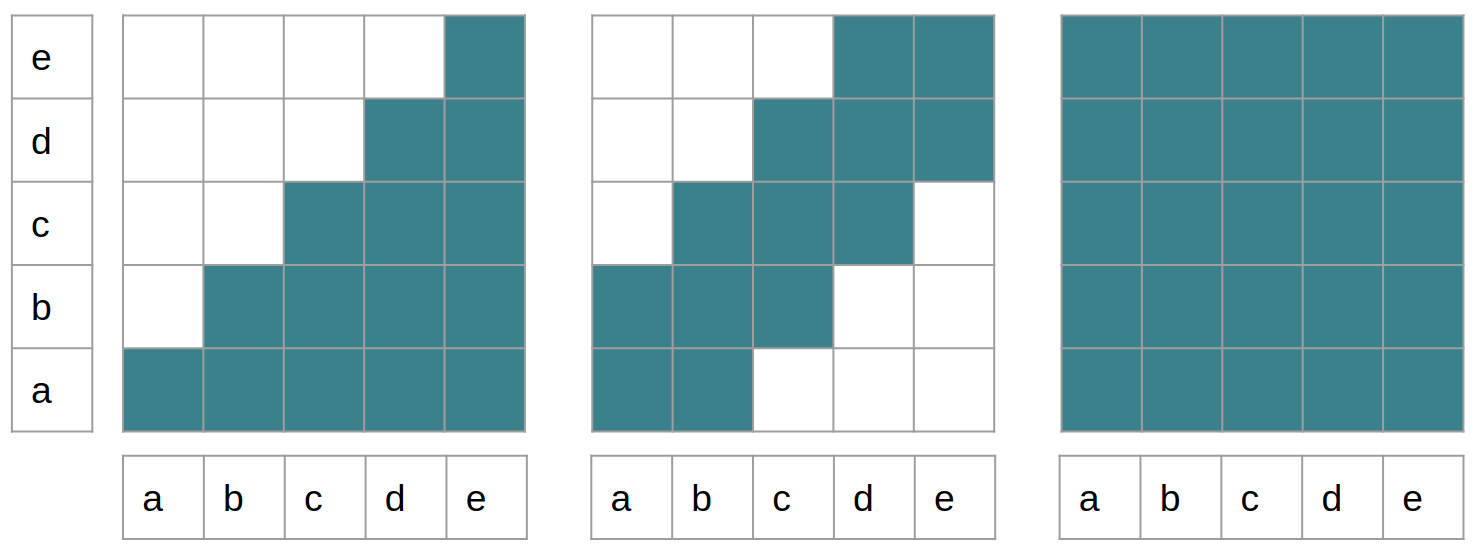
\includegraphics[width=\textwidth]{graphics/encoding.png}
\caption[Illustration of context range at each token in different encoding mechanism]{Illustration of context range at each token in different encoding mechanism. From left to right: Recurrent encoder, Convolutional encoder, Attention-based encoder. The example sequence is $[a,b,c,d,e]$ and each colored column represent the context range of the corresponding token.}
\label{fig:encoding}
\end{figure*}

The decoder works similarly to a language model as it predicts one token per time step. However, the decoder conditions its prediction on the source sequence. Therefore, the decoder takes the output of the encoder as its inputs. An Auto-regressive decoder conditions its prediction on the predictions of previous steps and the source sequence. Because all of our experiments use auto-regressive NMT, from now, a decoder is an auto-regressive decoder if there is no other specification. The decoder usually uses the same neural architecture as the encoder. However, unlike the encoder, the range of context of a token is strictly limited to its preceding tokens. Because the hidden state of the decoder is computed from the previous hidden states and the observation of the previous step, we need to initialize the $0^{th}$ hidden state $s_0$ (optional) and the $0^{th}$ token. That is why we always begin the target sequence by the token $<BOS>$, and the decoder starts predicting from the second token. For example, if $[a,b,c,d,e]$ is predicted by the decoder, the prediction of token $a$ is conditioned by source sequence $x$ and $<BOS>$; the prediction of token $b$ is conditioned by source sequence $x$ and $[<BOS>,a]$, etc.. Besides, the decoder needs a signal to stop its generative prediction. We always end a prediction by "end-of-sentence" token or $<EOS>$. Therefore, instead of predicting $[a,b,c,d,e]$, the decoder predicts $[a,b,c,d,e, <EOS>]$. Concerning the construction of hidden states, the Recurrent decoder usually initializes $s_0$ by the last hidden state of the encoder followed by a linear transformation. In contrast, the Convolutional decoder and the Attention-based decoder do not need to initialize $s_0$ as every hidden state directly accesses the predictions preceding its time step without going through its preceding state. We illustrate the difference between decoding paradigms in the figure \ref{fig:decoding}.

\begin{figure*}[htbp]
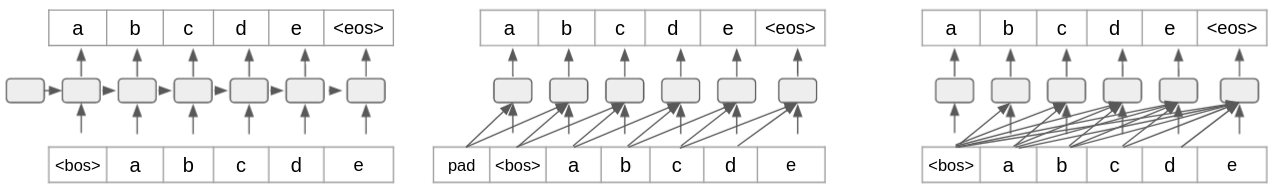
\includegraphics[width=\textwidth]{graphics/decoding.png}
\caption[Illustration of 3 most popular auto-regressive decoding paradigms]{From left to right: Recurrent decoder, Convolutional decoder, Attention-based decoder. The example sequence is $[a,b,c,d,e]$. The figure illustrates only one layer of the decoder.}
\label{fig:decoding}
\end{figure*}

NMT's Encoder/Decoder is usually a stack of multiple layers. As described above, the input source sequence is mapped to a sequence of word embeddings. This is considered as $0^{th}$ layer of the Encoder. The $i^{th}$ layer is built upon the $(i-1)^{th}$ layer by applying the same encoding mechanism (recurrent layer, convolutional layer or self-attention layer) to the output of the $(i-1)^{th}$. For example, \cite{Vaswani17attention} stacks 6 Transformer layers in both the encoder and the decoder of the NMT model. Deep NMT models are able to learn from very large-scale of parallel data \cite{Ott18scaling} and continually create new state-of-the-art performances. However Deep NMT models are harder to train because the gradient flow has to back-propagate through many layers. In order to prevent the gradient flow from vanishing, which happens when the value of the output of the linear transformation in some layer jumps outside the domain of the activation function, \citep{He16deep} proposes using residual connections, which replaces $f(x)$ by $f(x)+x$ where $x$ is the output of the lower layer and $f(.)$ is the transformation of the layer, to transit from the lower layers to their following layers. By using residual connections, a fraction of the gradient still reaches the lower layer and continues to propagate until the lowest layer.

Deep NMT models also suffer from Internal Covariate Shift in which the distribution of the value of each layer significantly changes due to the change of the parameters of the models. In deep network, the distribution of the value of high layers is highly affected the parameters of the lower layers and can be dramatically shifted by a small change in the value of those parameters. Large shift can push the value of the layer to the saturation zone of activation function where the gradient is extremely small. In practice, the saturation problem can be mitigated by using Rectified Linear Units $RELU(x) = max(x,0)$ \cite{Nair10rectified}. Recently, \cite{Ioffe15batch,Jimmy16layer} propose different normalization methods to stabilize the value of layers so that they are not easily pushed to saturation zone of activation function. In principle, Normalization methods re-scale and re-center the distribution of the value of each layer with learnable mean and learnable variance. Normalization methods prove to be very helpful in practice. For example, Layer normalization must be included in every layer of Attention-based NMT \cite{Vaswani17attention}.

\begin{figure*}[htbp]
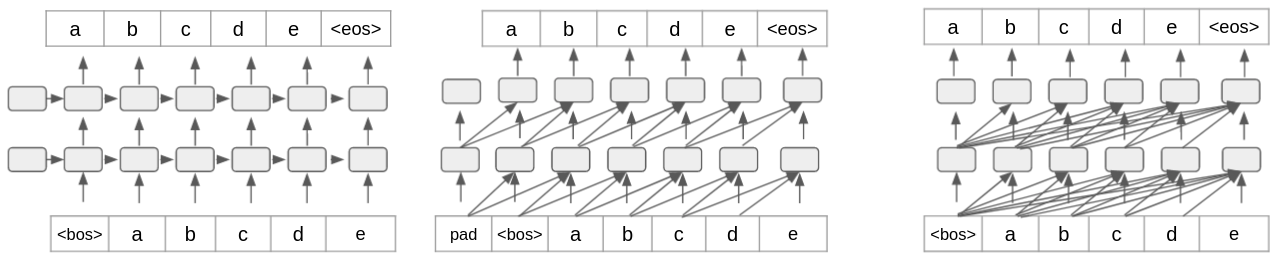
\includegraphics[width=\textwidth]{graphics/multi_layer_decoder.png}
\caption[Illustration of 3 most popular multi-layer auto-regressive decoding paradigms]{From left to right: Recurrent decoder, Convolutional decoder, Attention-based decoder. The example sequence is $[a,b,c,d,e]$. The figure illustrates only two layers of the decoder.}
\label{fig:decoding}
\end{figure*}

\section{Recurrent NMT} \label{sec:rrn}
\nomenclature[rnn]{RNN}{Recurrent neural network}
This section reviews the very first NMT architecture the Recurrent Neural Network (RNN). Recurrent NMT (\nomenclature[rnmt]{RNMT}{Recurrent neural machine translation}) is composed of a Recurrent encoder, a Recurrent decoder and tables of word embeddings. Recurrent encoder and Recurrent decoder usually use the same type of layer such as Gated recurrent unit (GRU) and Long-short term memory (LSTM), which we will explain in the following section. Recurrent NMT is strictly auto-regressive as each hidden state in encoder/decoder has to go through every intermediate state to assess the information of any time step before it. The hidden states of RNMT inherit the information of the order, which is an advantage before Convolutional NMT and Attention-based NMT, from this encoding paradigm. However, lack of straightforward accesses to positions of the input sequence causes many difficulties to the training of RNMT.

\subsection{GRU, LSTM layers}
\nomenclature[gru]{GRU}{Gated recurrent unit}
\nomenclature[lstm]{LSTM}{Long-short term memory}
Gated recurrent unit (GRU) and Long-short term memory (LSTM) are the 2 most popular layers in the group of Recurrent neural network. They follow the auto-regressive paradigm by constructing the hidden states one by one as follows.
\begin{equation}
\begin{array}{rcl}
h^l_t = f(h^{l-1}_t, h^l_{t-1})
\end{array}
\end{equation}
Where $h^{l-1}_t$ is the hidden state at time step $t$ of the $(l-1)^{th}$, $0^{th}$ layer is the sequence of word embeddings; the mapping f can be GRU cell or LSTM cell, which will be explained below.

LSTM was first introduced \cite{Hochreiter97long}, uses 4 gating functions including input gate i, output gate o, forget gate f and memory cell c. At each time step t, the contextualized embedding $h_t$ is computed as follows.
\begin{equation}
\label{eq:lstm}
\begin{array}{rcl}
f_t &=& \sigma_g (W_f h^{l-1}_t + U_f h_{t-1} + b_f)\\
i_t &=& \sigma_g (W_i h^{l-1}_t + U_i h_{t-1} + b_i)\\
o_t &=& \sigma_g (W_o h^{l-1}_t + U_o h_{t-1} + b_o)\\
\tilde{c}_t &=& \sigma_c (W_o h^{l-1}_t + U_o h_{t-1} + b_o)\\
c_t &=& f_t \odot c_{t-1} + i_t \odot \tilde{c}_t\\
h_t &=& o_t \odot \sigma_h(c_t)\\
\end{array}
\end{equation}
where $\sigma_g$ is sigmoid function, $\sigma_c$ is hyperbolic tangent function, $\sigma_h$ is either hyperbolic tangent function or identity function and $\odot$ is element-wise multiplication. These functions are applied element-wise to intermediate vectors in the equations.

The motivation behind this highly complex structure is to stabilize the exploding/diminishing gradient flow \citep{Pascanu13onthe} conduceted by back-propagation through time (BPTT \nomenclature[bptt]{BPTT}{Back-propagation through time}) \cite{Hochreiter97long}. The second architecture GRU, which was proposed by \cite{Cho14properties}, mitigates the complexity of LSTM by using only three gates as follows.
\begin{equation}
\label{eq:gru}
\begin{array}{rcl}
z_t &=& \sigma_g (W_z h^{l-1}_t + U_z h_{t-1} + b_z)\\
r_t &=& \sigma_g (W_r h^{l-1}_t + U_r h_{t-1} + b_r)\\
\hat{h}_t &=& \sigma_h (W_h h^{l-1}_t + U_h (r_t \odot h_{t-1}) + b_h)\\
h_t &=& (1-z_t)\odot h_{t-1} + z_t \odot \hat{h}_t\\
\end{array}
\end{equation}
Where $\sigma_h$ is a hyperbolic tangent function while other notations are the same as in the equations \ref{eq:lstm}.
\subsection{RNN encoder}
RNN encoder uses LSTM or GRU layer to encode the source sequence. RNN encoder can use more than one layer to capture more fine-grained language representation \cite{Li20shallow}. The $0^{th}$ layer is a sequence of word embeddings, which are extracted from the look-up table of the source side using the indices provided by the source sequence. 

\subsubsection{Bidirectional RNN encoder}
Unlike the decoder, the encoder is not obliged to process the input sequence from left to right. Effectively, the context of one token in the source sequence contains not only its preceding neighbors but also its following neighbors. Therefore, encoding the source sequence from left to right is not enough to cover the context of each token. To increase the coverage of contextualized embedding, the encoder process the source sequence both from left to right and from right to left at the same time, therefore becomes a bidirectional encoder. Bidirectional encoding results in two sequences of contextualized embeddings; the encoder simply combines two contextualized embeddings of a token into one real vector via either concatenation or summation. The resulting contextualized embedding captures information of every word in the source sequence around its corresponding token. 
\subsection{RNN decoder}
RNN decoder predicts the target sequence from left to right, one token per time step. It initializes the $0^{th}$ hidden state by zero vector or a linear transformation of the last hidden state of the last layer of the encoder. 
\subsubsection{Attention mechanism \label{ssec:attention}}
Attention mechanism consists 3 components: Query vectors, Key vectors and Value vectors. Given a sequence $Q_i$, $i \in [1 \cdots n]$, $K_j$, $j \in [1 \cdots m]$ and $V_j$, $j \in [1 \cdots m]$, the results
of the attention mechanism composed by those vectors will be as follow.
\begin{equation}
Attention(Q,V,K)_i = \displaystyle{\mathop{\sum}_{j=1}^{m}} \frac{exp(sim(Q_i,K_j))}{\displaystyle{\mathop{\sum}_{p=1}^{m}}exp(sim(Q_i,K_p))}*V_j, i \in [1, \cdots, m]
\end{equation}
Where function $sim(x,y)$ can be a simple dot product $<x,y>$ \citep{Vaswani17attention}, a generalized dot product $<x,W_a*y>$ or $<v_a,tanh(W_a*[x,y])>$ \citep{Luong15stanford, Bahdanau15learning}.

The attention mechanism manages and quantifies the dependence between the input sequence and the output sequence (e.g., source contextualized embeddings and target contextualized embeddings), or the input sequence itself (e.g., self-attention layers in Transformer \citep{Vaswani17attention}). In the RNN MT model, the attention mechanism is used to capture the dependence of each token in the target sequence on the tokens in the source sequence. For example, \cite{Bahdanau15learning} computes a context vector at $i^{th}$ time step in the decoder as follows.
\begin{equation}
\begin{array}{rcl}
c_i &=& \sum_{j} \alpha_{ij} h_j \\
\alpha_{ij} &=& \frac{exp(e_{ij})}{\sum_{k}exp(e_{ik})} \\
e_{ik} &=& sim(s_{i-1},h_k)\\
\end{array}
\end{equation}
where $h_j$ is the output of the last layer of the encoder, $s_{i-1}$ is the hidden state at $(i-1)^{th}$ time step of the last layer of the  decoder. This context vector will be used to compute the hidden state at $i^{th}$ position by Attention mechanism improves the translation quality of very long sequences. Indeed, the context vector produced by the RNN encoder struggles to capture all the dependence between tokens  of the input sequence because it lacks the direct links between 2 tokens. The information of a token vanishes while the encoder moves toward the far ending of the input sequence. The same problem happens with the decoder when it decodes the context vector into the output sequence. The attention mechanism provides the direct links from each output token to any input token, allows the decoder to capture the information of any input token regardless of its position.

\section{Convolutional NMT} \label{sec:cnn}
\nomenclature[cnn]{CNN}{Convolutional neural network}
Convolutional neural network was successfully applied to MT task in the work of \citet{Ghering17convolutional} that outperformed the current state-of-the-art performance of the RNN MT. As we aforementioned above, Convolutional MT does not construct the hidden states iteratively in one direction but considers the sequence as an image, of which each column of pixel is a word embedding, and applies convolutional kernels on it.
\subsection{Convolutional encoder}
Concretely, each layer of Convolutional encoder contains an one dimensional convolution kernel followed by a non-linearity. We denote $h^l_i$ the $i^{th}$ hidden state of $l^{th}$ layer. Those hidden states are computed as follows.
\begin{equation}
\begin{array}{lcr}
h^l_i = v\bigg( W^l \big[h^{l-1}_{i-\frac{k}{2}}, \cdots, h^{l-1}_{i+\frac{k}{2}} \big] + b_w \bigg) + h^{l-1}_{i}
\end{array}
\end{equation}
Where $W^l \in \mathbb{R}^{2d \times kd}$, $b_w \in \mathbb{R}^{2d}$, d is the dimension of hidden states as well of word embeddings, k is the width of the kernel, the activation function v is Gated Linear Unit \citep{Ghering17convolutional}, that is described in the following equation.
\begin{equation}
\begin{array}{lcr}
v([A,B]) = A \odot \sigma(B)
\end{array}
\end{equation}
Where $\odot$ is element-wise multiplication, $\sigma$ is sigmoid function.
\subsection{Convolutional decoder}
Unlikely the Convolutional encoder, in which each hidden states has access to its left and right neighbors, the decoder only allows left accesses to avoid conditioning the predictions on the following tokens, which will not exist before the prediction in the inference. Therefore, citet\{Ghering17convolutional} appends $k-1$ padding tokens in the left side of the output sequence, e.g $PAD$, $PAD$,$ <BOS>$,$je$,$t'$,$aime$ for convolution kernel of size 3 so that $\big[ PAD, PAD, <BOS>\big]$ predicts $je$, $\big[ PAD,<BOS>,je\big]$ predicts $t'$ etc.
In the decoder, Convolutional NMT model also uses attention mechanism to improve the performance on the long sentences. \\citet{Ghering17convolutional} propose a version slightly different from ones of \citet{Luong15stanford, Bahdanau15learning}. For each $l^{th}$ decoder layer, the query will be a combination of the hidden state $h^l_i$ and the word embedding of the previous token $g_i$.
\begin{equation}
\begin{array}{rcl}
d^l_i = \W^l_dh^l_i + b^l_d + g_i
\end{array}
\end{equation}
The keys are still the hidden states of the last layer of the encoder $z^u_j$. The values are the combinations of the hidden states $z^u_j$ and the word embedding $e_j$. The score attention is simply dot product between the query vector and the key vector followed by softmax function.
\subsection{Positional embedding}
\citet{Ghering17convolutional} propose using embeddings corresponding to each position of the input sequence in order to equip the Convolutional NMT model with a sense of order as Convolution kernel does not take in account the order of tokens in the input sequence. Effectively, if we interchange the position of tokens outside the window of the kernel, the value of the hidden state does not change. Positional embeddings are real value vector having same dimension as word embeddings. Positional embeddings are added to word embeddings of the corresponding position before passing to the first layer.

\section{Attention-based NMT} \label{sec:transformer}
Transformer architecture was first introduced by \cite{Vaswani17attention} and has quickly become the state-of-the-art architecture not only in MT but also in language modeling (LM)\cite{Devlin19bert,Brown20language,Conneau19cross}, text summarization \cite{Zhang20pegasus} etc. The Transformer model's power relies on the attention mechanism, which was discussed in the previous section \ref{ssec:attention}. The Transformer model consists of a fully attention-based encoder and decoder. 
\subsection{Transformer encoder}
The Transformer encoder consists of layers made of a multi-head self-attention sub-layer followed by a position-wise fully connected feed-forward network. The multi-head self-attention sub-layer is an extension of the self-attention sub-layer and is described by the following equation.
\begin{equation}
\begin{array}{rcl}
MultiheadAttention\big( Q,V,K \big) &=& Concat \big[ head_0, \cdots , head_h \big] W_0\\
head_i &=& Attention \big( QW_i^Q, VW_i^V, KW_i^K \big)\\
\end{array}
\end{equation}

Where $W_i^Q, W_i^V, W_i^K \in \mathbb{R}^{d_k \times d_h}$ with $d_h \times h = d_k$, $d_k$ is the dimension of word embedding space and also the size of Transformer model. Unlike the version in the section \ref{ssec:attention}, the attention mechanism is simply as follows.
\begin{equation}
Attention\big( Q, V, K \big) = Softmax\big(\frac{Q K^T}{\sqrt{d_k}} \big) V
\end{equation}
The feed-forward network is designed as follows.
\begin{equation}
FFN(x) = ReLu(xW_1+b_1)W_2+b_2
\end{equation}
Where $W_1 \in \mathbb{R}^{d_k \times d_b}$,$W_2 \in \mathbb{R}^{d_b \times d_k}$,$b_1 \in \mathbb{R}^{d_b}$,$b_2 \in \mathbb{R}^{d_k}$.
The final detail is that the output of each sub-layer has to pass through a Layer-Normalization sub-layer \citep{Jimmy16layer}. In conclusion, the contextualized embedding of the $l^{th}$ layer of the Transformer encoder will be as follows.
\begin{equation}
\begin{array}{rcl}
\tilde{h}^l &=& LN\bigg(Multihead\big(h^{l-1}, h^{l-1}, h^{l-1}\big) + h^{l-1}\bigg) \\ 
h^l &=& LN\bigg(FFN\big(\tilde{h}\big) + \tilde{h}\bigg)
\end{array}
\end{equation}
Where $LN$ is a Layer-Normalization sub-layer.
\subsection{Transformer decoder}
The Transformer decoder consists of layers made of a multi-head self-attention sub-layer followed by a multi-head cross-attention sub-layer then by a position-wise fully connected feed-forward network. The multi-head self-attention sub-layer and the feed-forward network have the same design as those in the Transformer encoder. The multi-head cross-attention sub-layer of the $l^{th}$ layer of the decoder uses the output of the last layer of the encoder as keys and values, the output of the $l^th$ self-attention sub-layer as queries.
\begin{equation}
\begin{array}{rcl}
\tilde{s}^l &=& LN\bigg( Multihead\big( s^{l-1},s^{l-1},s^{l-1} \big) + s^{l-1} \bigg) \\
\bar{s}^l &=& LN\bigg( Multihead\big( \tilde{s}^l, h^u, h^u \big) + \tilde{s}^l \bigg) \\
s^l &=& LN\bigg( FFN\big( \bar{s}^l \big) + \bar{s}^l \bigg) \\
\end{array}
\end{equation}
where $s^l$,$s^{l-1}$ are the outputs of the $l^{th}$ and $(l-1)^{th}$ layers of the decoder respectively, $h^u$ is the output of the last layer of the encoder.

In order to prevent the future information in the decoder, at each time step $i^{th}$, the attention scores of tokens at positions after $i^{th}$ are masked by zero.

\subsection{Positional embedding}
Similar to the Convolutional encoder/decoder, the Transformer encoder/decoder does not respect the order of tokens as it fully connects every pair of tokens in parallel. In order to represent the position of tokens in the sequence, \cite{Vaswani17attention} proposed the use of positional embedding. Unlike \citet{Ghering17convolutional}'s positional embedding, this version is not parameterized as given the size of word embedding $d_k$ , the positional embedding of position $i^{th}$ is defined as follows
\begin{equation}
\begin{array}{rcl}
PE\big(pos,2i\big) &=& sin \big( \frac{pos}{1000^{\frac{2i}{d_k}}} \big)\\
PE\big(pos,2i+1\big) &=& cos \big( \frac{pos}{1000^{\frac{2i}{d_k}}} \big)\\
\end{array}
\end{equation}
The positional embedding will be added to the corresponding word embedding of the $i^{th}$ token of the input sequence.
\section{NMT training} \label{sec:train}
The values of the parameters in the NMT model is estimated by gradient descent method \citep{Nesterov14introductory}, which is one of the oldest approaches in the Optimization area \citep{Cauchy1847method}. The loss function is the traditional cross-entropy of the training data. 
\begin{equation}
L(\theta) = -\displaystyle{\mathop{\sum}_{x,y}}log P(y|x;\theta)
\end{equation}
The gradient is computed by back-propagation algorithm \citep{Rumelhart88learning}. Like many deep learning models, the NMT model is usually trained with a massive amount of data that makes the gradient descent method is not computationally plausible. Therefore, stochastic gradient descent is proposed to mitigate the computational burden of large-scale models \citep{Herbert51stochastic,Kiefer52stochastic,Bottou10large}. However, Deep Neural networks are usually much harder to train because of their size and their complex structure \cite{Pascanu13onthe,Glorot10understanding}. Many approaches are proposed to facilitate the training of deep models such as Gradient clipping \citep{Pascanu13onthe}, Truncate back-propagation \citep{Jaeger02tutorial}, Normalization methods \citep{Ioffe15batch,Jimmy16layer}, Residual connections \citep{He16deep}, Noam schedule \citep{Vaswani17attention} etc.

\section{Decoding algorithm} \label{sec:inference}
The NMT model basically models the conditional probability $P(y|x)$of the translation sentence $y$ given the input sentence $x$. The prediction of the NMT model is the sentence with the highest conditional probability.

\begin{equation}
\hat{y} = \displaystyle{\mathop{\argmax}} P(y|x;\theta)
\end{equation}

However, the search space of $y$ is infinitely large, causing the implausibility of the exact search. Beam search \citep{Och98improving} is the most common decoding algorithm in Neural Machine Translation and Statistical Machine Translation. 

Beam search starts with K empty hypotheses, which are initialized by "begin of sentence" token $<BOS>$. For the $i^{th}$ current hypothesis $[y^{i}_{<t}]$, the top-K tokens, with the highest conditional probabilities $P(y_t = a_i | y_{<t},x;\theta)$, are picked and appended to the current hypothesis. The search space, therefore, is extended to $K*K$ hypotheses. Beam search selects only the top $K$ hypotheses from these $K*K$ hypotheses. Beam search stops extending the completed hypotheses, which are ended with the "end of sentence" token $<EOS>$ or reach the predefined length limit. Beside the left-to-right decoding, there are several variant decoding direction including non-monotonic decoding \citep{Welleck19non}, non auto-regressive decoding \citep{Jiatao17non}, synchronous bidirectional decoding \cite{Zhou19synchronous}. Because the decoding algorithms are not included in this research topic, we would like to be limited to this brief description.
\nomenclature[eos]{EOS}{end-of-sentence}

\section{MT evaluation}
\subsection{BLEU, sacreBLEU}
\subsection{Domain errors}






































